%!TEX root = ../report.tex

\chapter{Introduction}

\section{Densenet}

In Densenet each layer connects to every layer in a feed-forward fashion. 
With the basic idea to enhance the feature propagation, each layer of Densenet blocks takes the feature-maps of the previous stages as input.  
\begin{figure}[ht]
\centering
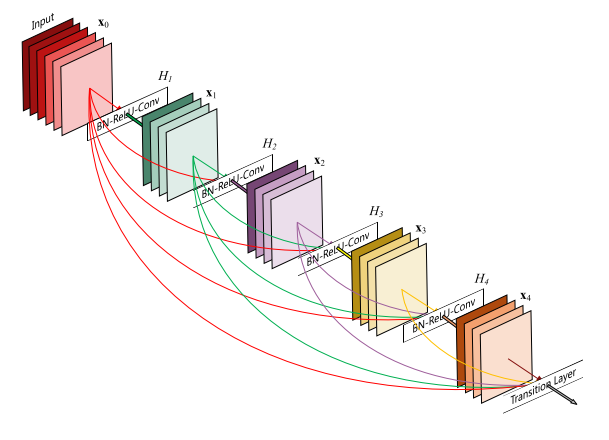
\includegraphics[width=0.5\textwidth]{images/densenet/densenet.png}
\caption{\label{fig:densenet}Densenet structure.}
\end{figure}
\flushbottom
\newpage
\subsection{Siamese Densenet structure}

Where the branches of the Siamese network are Densenet. 
% Commands to include a figure:
\begin{figure}[ht]
\centering
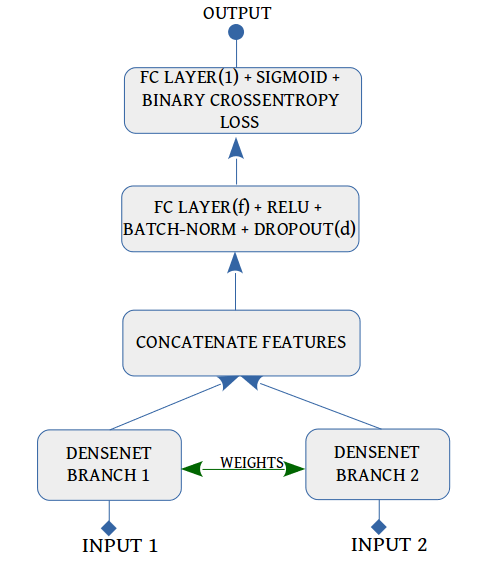
\includegraphics[width=0.5\textwidth]{images/densenet/siamese_densenet_structure.png}
\caption{\label{fig:dn_siamese}Siamese Densenet structure.}
\end{figure}

\section{Hyper-parameters}
Hyper-parameters are those parameters whose values are set before the training, unlike other parameters whose values are learned during the training. 
For example learning rate, batch size. \cite{wikihyper}
\subsection{Parameters of Densenet}
\begin{itemize}
  \item \textbf{Growth rate}: Number of filters to add per dense block. Growth rate regulates how much information is contributed by each layers to the global state. 
  Global state is the collective knowledge of the network, that is the state of the previous layers are flown into each layer in form of feature-maps, 
  which is considered as global state. Each layer adds k more feature-maps to the current state, when growth rate is k.

  \item \textbf{Nb\_filter}: initial number of filters. -1 indicates initial number of filters will default to 2 * growth\_rate.

  \item \textbf{Nb\_layers\_per\_block}: number of layers in each dense block. Can be a -1, positive integer or a list. If -1, calculates nb\_layer\_per\_block from the network depth. 
  If positive integer, a set number of layers per dense block. If list, nb\_layer is used as provided. Note that list size must be nb\_dense\_block.

  \item \textbf{Depth}: number or layers in the DenseNet.

  \item \textbf{Nb\_dense\_block}: number of dense blocks to add to end.

  \item \textbf{Bottleneck Layers}: To improve computation efficiency a bottleneck layer with 1x1 convolution is introduced before each 3x3 convolution layers. 
  \item \textbf{Compression}: Reduces the feature maps in transition layers and makes the model more compact and computationally efficient.
\end{itemize}

\begin{figure}[ht]
\centering
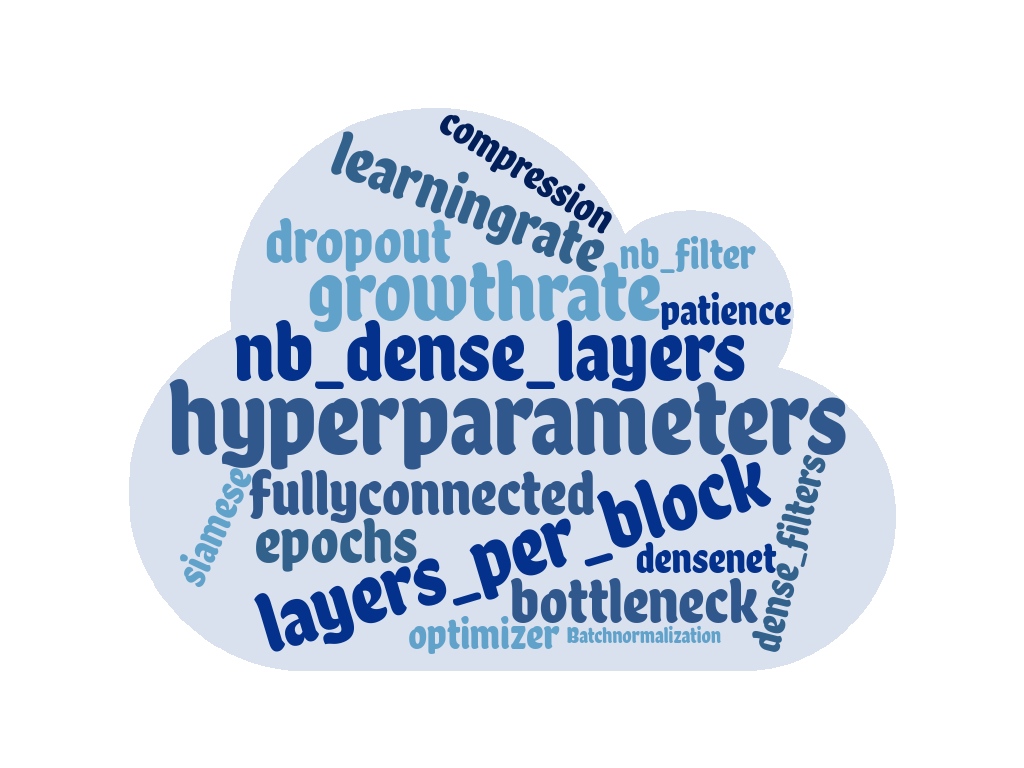
\includegraphics[width=0.5\textwidth]{images/densenet/wordcloud_hyperparameters.png}
\caption{\label{fig:wordcloud_hp}Hyper parameters word cloud.}
\end{figure}

\subsection{Other hyper-parameters}
After concatenation of the features from the Densenet branches, the merged features need to pass through a small network figure \ref{fig:dn_siamese} before being connected to the 
last layer with Sigmoid activation function and single output for binary classification. Afore mentioned small network from consists of a dense layer, followed by a Batch 
normalization layer and Relu activation layer respectively. After this a Dropout layer is added to ensure better generalization. So the parameters such as the filter size 
of the Densenet(f) and Dropout value (d) are the main hyper-parameters related to network barring the Densenet branches. Apart from these, there are other general hyper-parameters
such as learning rate, batch size for training, optimizer. 

\section{Grid search method}
Currently the search space for the evaluation is hand designed and supplied to the evaluation script externally. Example
\begin{figure}[ht]
\centering
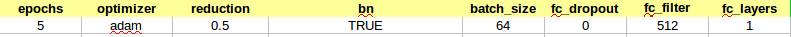
\includegraphics[width=1\textwidth]{images/densenet/test_cases.png}
\caption{\label{fig:search_space}Custom grid search space example.}
\end{figure}


\begin{itemize}
 \item Each test cases are evaluated 5 times.
 \item Dataset is divided into three parts, Train ( 31K) Validation(7K) Test(7K). Note: Validation data in keras does not contribute to training, 
 but it can affect training indirectly through Earlystop and ReduceLROnPlateau
 \item Output: ROC AUC score is calculated on the prediction on test data. The mean auc, standard deviation and Maximum auc is presented out of n trials. 
 Also the number of parameters are reported.
\end{itemize}

\subsection{Disadvantages}
In cutting edge algorithms for hyper parameter tuning like \textbf{TPE(Tree-structured parzen estimator)}
Sequentially construct models to approximate hyperparameters based on previous measurements. Hence the search time for finding the best parameters are significantly lesser than 
simple grid search.
This was the first choice method. But fails after some trial of evaluation with memory related error, \textbf{bad\_alloc}. This issue could not be fixed even after decreasing 
the batch size to 2/4 or clearing the keras backend session.

\subsection{Advantages} 
More control over the testing conditions for different networks, for example hand tuning the epochs for different architectures to ensure they train well.
Whole search space can be cut into smaller parts and run in parallel.

\subsection{Grid search strategy}
Since there are lot of parameters, practically, infinite test cases might be designed. To keep the grid search focused and less computationally expensive it makes sense to 
first search for coarser grid of parameters rather than very fine ones. When and if a bracket of parameters are shortlisted which works better than others, the finer parameter
search will be performed only specific to those range of parameters and not the whole grid.

\section{Results} 

\subsection{Coarse grid search on Densenet hyper-parameters}
For the estimation of the best performing parameters of Densenet for the branches of the Siamese, first a coarse grid search is been performed with 
\begin{itemize}
 \item Layers per block are chosen among 2,3,4,5,6. For single dense block evaluation goes up-to 12 layers. More than that(14) causes memory to run out as the size gets too big 
 for the cluster gpu memory(16GB). 
 \item Each network has been evaluated for growth rates of 6,12,18,24,30,36. 
 \item Different dense block sizes of 1,2,3,4.  
 \item Not all the possible combinations has been evaluated as quite extensive as possible
 \item The basic idea here is to narrow down the possible network sizes from the Densenet parameters perspective. There are other parameters but number of dense block, 
 growth rate and layers per block are three main parameters which controls the architecture/size of the network the most.
 \item The parameters compression/reduction and bottleneck are set 0.5 and True respectively because both this parameters controls the compactness of the model and help 
 reducing the parameter required, hence in theory enabling us to evaluate much bigger networks. So the network that is being evaluated here are named Densenet-BC by authors, 
 I.e Densenet with bottleneck and compression.
 \item For more fine grained analysis the compression and bottleneck parameters will also be evaluated. 
 \item nb\_filter values are fixed at 16 for this test
 \item The parameter classes are set to 2, which represents 1 for matching and 0 for not-matching pairs
 \item 96,96 is the input image dimensions. And it’s single channel. So depending on local setting of the keras, “channel-first” or “channel-last” suitable input\_shape is 
 chosen automatically as  1,96,96  or 96,96,1 respectively.
 \item The learning rate used for the test was 2E-4
 \item Dropout for Densenet used as 0.2 to handle over-fitting.  
 \item Epochs are different for different architectures to ensure that the networks are able to achieve at least 95\% training accuracy. 
 \item From the keras side of the parameters, after concatenating the Densenet branch output feature maps, the “combined features” then passed through a fully-connected  
 layer of 512 filter size, which is followed by Relu activation and Batchnormalization(BN)  and then a dropout(0.5) has been added to ensure better generalization. 
 \item Some of this values needs to be further evaluated as well, how ever current values were obtained using some of manual tuning and assumed to be a decent starting point.
 \item Flatten is used as pooling at the end of the Densenet, it is introduced by this work which replaces the Globalaveragepooling step with a flatten. This causes increase 
 in parameters overall though.
 \item Binary\_crossentropy loss function with sigmoid activation function used for the binary classification, this final layer acts as the binary classifier.
 \item In all the cases the networks are being trained from scratch. The weights = None ensures that no previously trained weights are used.
\end{itemize}

\subsection{Coarse grid search parameters summary}
\subsubsection{Fixed hyper-parameters}
\begin{itemize}
 \item Nb\_filter: 16
 \item Subsample initial block: True
 \item Weights : None
 \item Dropout rate : 0.2
 \item Include top : False
 \item Compression : 0.5
 \item Bottleneck : True
 \item Pooling : \textbf{Flatten}
 \item Transition pooling : max
\end{itemize}

\subsubsection{Varying Hyper-parameters}
\begin{itemize}
 \item \textbf{Nb\_layers\_per\_block}:
 \begin{itemize}
  \item \textbf{One dense block architecture (nb\_dense\_block=1):}\\
  '2', '3', '4', '6', '8', '10', '12'
  \item \textbf{Two dense block architecture (nb\_dense\_block=2):}\\
  '2-2', '2-3', '2-4', '3-3', '3-4', '3-5', '4-4', '6-6'
  \item \textbf{Three dense block architecture (nb\_dense\_block=3):}\\
  '2-2-2', '2-2-3', '2-3-3', '2-2-4', '2-3-4', '3-3-2', '3-3-3', '3-3-4', '3-4-4', '3-4-5', '3-3-6', '4-4-4', '4-4-2', '4-4-3', '4-4-6', '6-4-2', '6-6-3', '6-6-6'
  \item \textbf{Four dense block architecture (nb\_dense\_block=4):}\\
  '2-2-2-2', '3-3-3-3', '4-4-4-4', '6-6-6-6'
 \end{itemize}
 \item \textbf{Growth rate}:
  \begin{itemize}
  \item Thin layers: 6, 12, 18
  \item Thick layers: 24, 30, 36
 \end{itemize}
 
\end{itemize}
\flushbottom
\newpage

\subsection{AUC analysis}
Each network is trained from scratch and evaluated on test data 5 times. The metric for evaluation is Area under curve(AUC). 

Displaying below is the top 20 architectures (layers per dense block and growth rates) in terms of highest mean AUC on test data across 5 trials.  

\begin{figure}[ht]
\centering
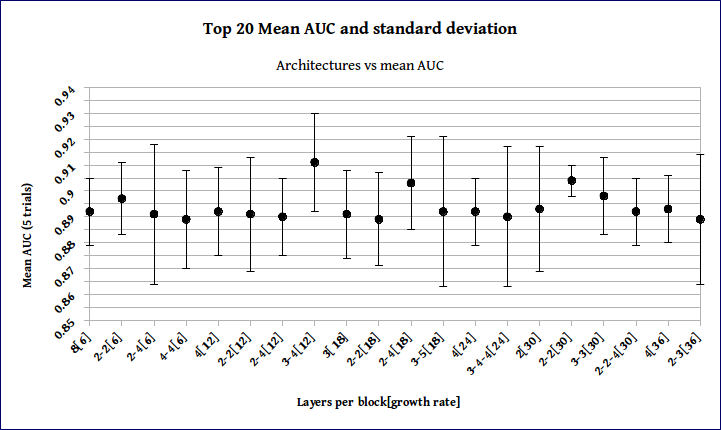
\includegraphics[width=0.5\textwidth]{images/densenet/auc_analysis_sortedby_growth.png}
\caption{\label{fig:meanAUC_growth}AUC analysis sorted by number of growth rate.}
\end{figure}

\begin{figure}[ht]
\centering
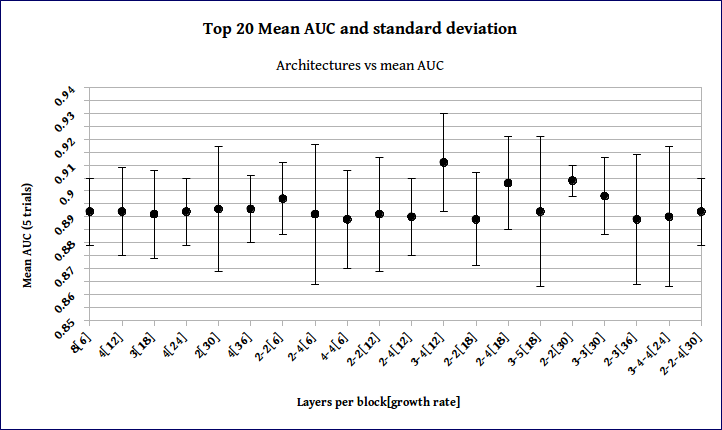
\includegraphics[width=0.5\textwidth]{images/densenet/auc_analysis_sortedby_denseblocks.png}
\caption{\label{fig:meanAUC_blocks}AUC analysis sorted by number of dense blocks.}
\end{figure}
Conclusion: Inconclusive!!\\
\flushbottom
\newpage

Displaying below is the top 20 architectures (layers per dense block and growth rates) in terms of highest max AUC on test data across 5 trials. 
\begin{figure}[ht]
\centering
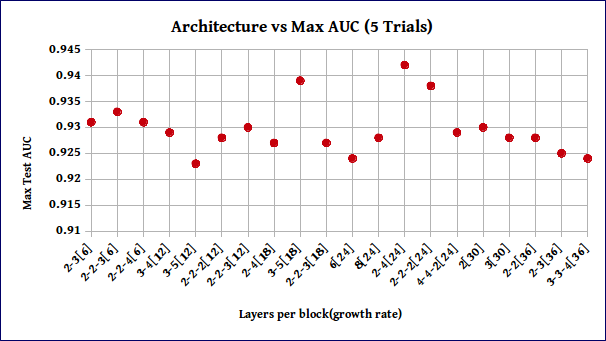
\includegraphics[width=0.5\textwidth]{images/densenet/auc_analysis_max_auc.png}
\caption{\label{fig:maxAUC_five}AUC analysis Maximum AUC.}
\end{figure}

\subsubsection{Conclusion}
\begin{itemize}
 \item It is clear from the top 20 performer across mean and max AUC analysis that the architectures consisting lesser layers per block outperforms networks with more layers per block in general. 
 \item The four dense block architectures did not make it to the top 20 in any of the case. Their performance on the test data is worse, so under current setup and assumptions they work worse.
 Even though they are able to train above 95\% train accuracy their generalization on the test data seems to be poor in general.
 \item Two dense block networks in general works best in terms of mean AUC of the 5 evaluations.
 \item In terms of max AUC score some of the Three block and one block Densenet works very good as well, but may not be that consistent in general and did not make it in the top 20 mean AUC list.
 \item Some networks though, like 2-2, 2-4, 3-4, 3-5, 3, 8, 2-2-4 etc are of special interest since they have featured in both the list of mean and max top 20 AUC.
\end{itemize}

\subsection{Optimal growth rate analysis}
It is also important to find out the best growth rate for each of the architectures(layers per block). For this purpose, the growth rate with mean AUC of test data in 5 trials has been selected,
the Best growth rates across architectures are displayed in the graph below:

\begin{figure}[ht]
\centering
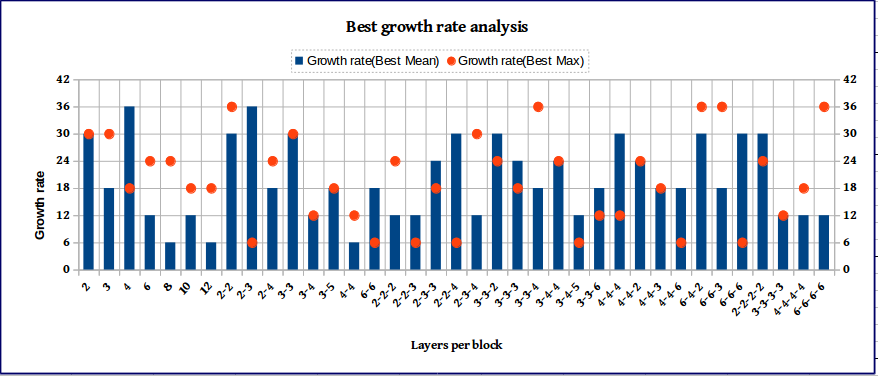
\includegraphics[width=1\textwidth]{images/densenet/best_growthrate_analysis.png}
\caption{\label{fig:best_growthrate}Architecture vs growth rate based on mean AUC.}
\end{figure}

But it is observed that the architectures with max AUC in 5 evaluations on test data. might consist of different growth rates than the one that displays best mean AUC. For this purpose, histogram of 
best performing growth rates obtained from mean and max AUC analysis is displayed in the figure below:

\begin{figure}
    \centering
    \begin{subfigure}[b]{0.4\textwidth}
        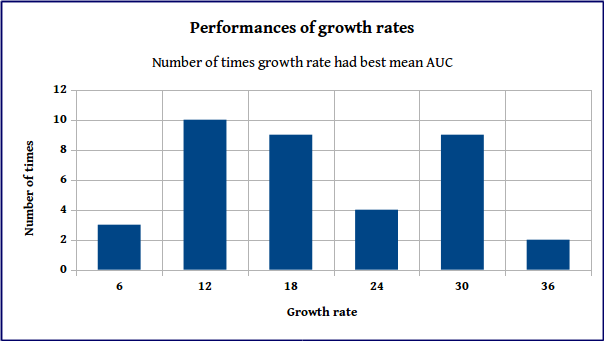
\includegraphics[width=\textwidth]{images/densenet/performances_of_growth_rates_mean_AUC}
        \caption{Histogram of growth rates depending on mean AUC}
        \label{fig:mean_auc_histogram}
    \end{subfigure}
    ~ %add desired spacing between images, e. g. ~, \quad, \qquad, \hfill etc. 
      %(or a blank line to force the subfigure onto a new line)
    \begin{subfigure}[b]{0.4\textwidth}
        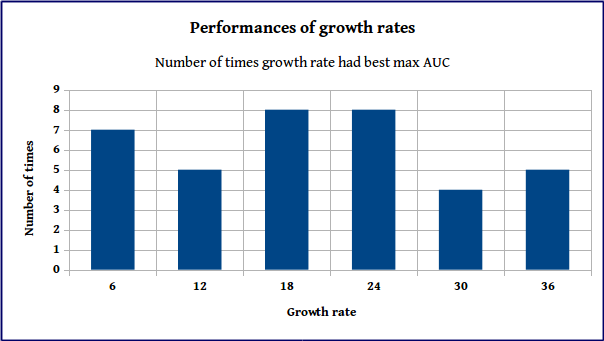
\includegraphics[width=\textwidth]{images/densenet/performances_of_growth_rates_max_AUC}
        \caption{Histogram of growth rates depending on max AUC}
        \label{fig:max_auc_histogram}
    \end{subfigure}    
    \caption{Cumulative growth rate analysis (histograms)}\label{fig:growthrate_histogram}
\end{figure}

\subsubsection{Conclusion}
\begin{itemize}
 \item It is evident from figure \ref{fig:max_auc_histogram}, based on the max AUC, there is no strong trend, its very random and inconclusive. Which is not very surprising given its just one run. 
With so many parameters and initialization and random dropouts involved, the network weights might learn very differently in spite of being trained in a same condition, resulting in a completely different decision boundary.
 \item In fgiure \ref{fig:mean_auc_histogram} it is visible that the contribution of growth rate 6 and growth rate 36 is really less, so probably they are too thin or too thick for the data. 
 \item From fgiure \ref{fig:growthrate_histogram} above it is safe to assume that growth rate 18 is very good performer in both analysis. Which also makes sense since it is neither too thin nor too thick. Because this conclusion 
 is based on just 5 evaluations of each architectures, we are open to experiment with other growth rates(except 6,36) as well for finer evaluation.
\end{itemize}

\subsection{Total parameters analysis}
\begin{itemize}
 \item It might be surprising but the single dense block networks have most parameters. This is also because of the flatten pooling that is used here in this work instead of global average pooling 2D. 
 \item And four block networks have the least total and trainable parameters. This is also supported by the theory in the paper
 \item How ever as the number of dense blocks keeps getting higher the non-trainable parameters also gets higher. So 4 blocks dense net has most number of non-trainable parameters.
 \item For the comparison 2, 2-2, 2-2-2, 2-2-2-2 blocks parameter sizes are compared below, all recorded for growth rate 18.
\end{itemize}

\begin{figure}
    \centering
    \begin{subfigure}[b]{0.4\textwidth}
        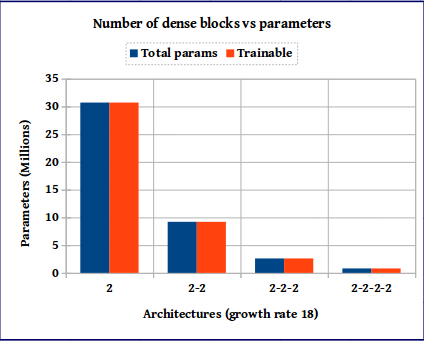
\includegraphics[height=5cm]{images/densenet/Denseblocks_vs_parameters}
        \caption{Parameters vs architectures}
        \label{fig:Denseblocks_vs_parameters}
    \end{subfigure}
    ~ %add desired spacing between images, e. g. ~, \quad, \qquad, \hfill etc. 
      %(or a blank line to force the subfigure onto a new line)
    \begin{subfigure}[b]{0.4\textwidth}
        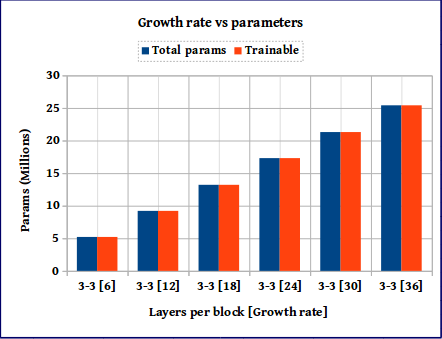
\includegraphics[height=5cm]{images/densenet/growthrate_vs_parameters}
        \caption{Parameters vs growth rates}
        \label{fig:growthrate_vs_parameters}
    \end{subfigure}    
    \caption{Total number of parameters analysis}\label{fig:total_parameters_densenet}
\end{figure}


\subsection{Standard deviation across blocks}
Another trend was observed that the standard deviation varies more as the number of dense blocks increases. 
So the std values for all the readings are collected for 1,2,3,4 number of dense blocks (nb\_dense\_blocks) separately and their mean values are presented in the table below.

\begin{figure}[ht]
\centering
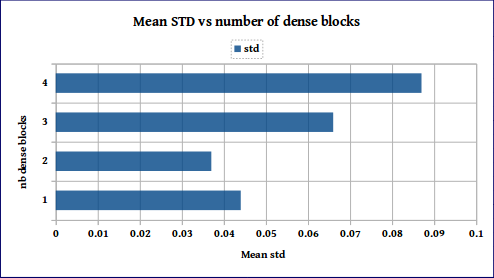
\includegraphics[width=0.6\textwidth]{images/densenet/std_vs_denseblocks.png}
\caption{\label{fig:std_vs_denseblocks} Mean Standard deviation vs number of dense blocks.}
\end{figure}

\begin{itemize}
 \item Even thought the number of sample size differs a lot [42,48,108,24] respectively for dense blocks 1,2,3,4  it does seem like standard deviation of AUC higher for dense block 3 and 4.
 \item It is probably because the blocks 3 and 4 networks have much lesser parameters than the 1 and 2 number of dense blocks.
\end{itemize}

\subsection{Finer grid search analysis}
\begin{itemize}
 \item From the first analysis the top 5 network based on mean AUC of 5 trials and top 5 network obtaining maximum AUC are further evaluated for 20 evaluations each. Other test conditions remain the same. 
 \item Results after 20 times evaluation are expected to be more dependable than 5 trials.
 \item In the chart below the mean AUC of 20 evaluations and its standard deviation is displayed in blue dots and black lines. 
 \item In red displayed the maximum AUC obtained in 20 evaluations
\end{itemize}

\begin{figure}[ht]
\centering
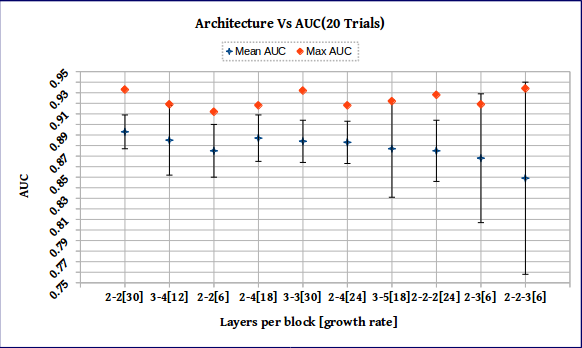
\includegraphics[height=5cm,width=0.7\textwidth]{images/densenet/arch_vs_auc_finer}
\caption{Finer search with top 10 architectures}
\label{fig:arch_vs_auc_finer}
\end{figure}

\begin{figure}[ht]
\centering
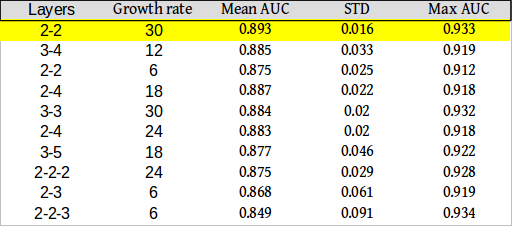
\includegraphics[height=3cm,width=0.5\textwidth]{images/densenet/finer_structure_analysis}
\caption{Finer search with 10 architectures}
\label{fig:arch_vs_auc_finer_table}
\end{figure}

\subsubsection{Conclusion}
\begin{itemize}
 \item It seems that in 20 evaluations layers 2-2 with growth rate 30 is the best result both in terms of lowest standard of deviation and highest mean AUC. As it happens its also second highest in terms of the 
 maximum AUC 0.933 just behind 0.934 from 2-2-3.
 \item 3-4, 2-4 networks are also performing well in terms of mean AUC. Their results are very close as well, so just evaluating 3-4 network for the finer analysis.
 \item 2-2-3 layers is interesting though, it has the highest standard deviation but 2 or 3 very good AUC scores too. So it needs to be further looked into.
\end{itemize}

\begin{figure}[ht]
\centering
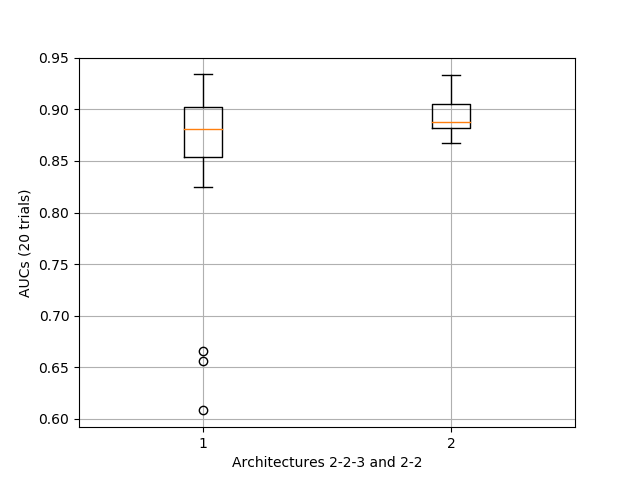
\includegraphics[width=0.5\textwidth]{images/densenet/arch_compare_boxplot.png}
\caption{Boxplot analysis architectures}
\label{fig:arch_compare_boxplot}
\end{figure}

in 2-2-3 analysis 3 AUC readings are detected as outliers out of 20 trials at 0.666, 0.608, 0.656
\begin{center}
 \begin{tabular}{||c c c c c c||} 
 \hline\hline
 Min & Q1 & Median & Q3 & Max & No. Outliers \\ [0.5ex] 
 \hline
 0.608 & 0.854 & 0.881 & 0.902 & 0.934 & 3 \\ 
 \hline
 0.867 & 0.882 & 0.887 & 0.905 & 0.933 & 0 \\
 \hline
\end{tabular}
\end{center}

The outliers are affecting the overall mean auc for 2-2-3 network, also causing big standard deviation. This outliers are probably caused by training getting stuck in local minima or similar. 2-2 is found to be more 
consistant, it has no outliers. It is believed that consistancy is desirable for a network. Hence 2-2-3 network is ruled out of contention for the best network, because of it's lack of consistancy.
\subsection{Nb\_filter analysis}
Initial number of filters. 8,16,32,64 are being evaluated here. Also a comparison between mean AUCs obtained from growth rate 18 and 30 is done under this analysis. Ten evaluations of each test cases has been done.
\begin{figure}[ht]
\centering
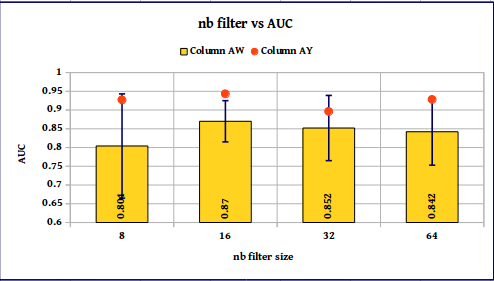
\includegraphics[height=4cm,width=0.5\textwidth]{images/densenet/nb_filter_vs_auc}
\caption{Nb\_filter vs mean AUC for growth rate 30}
\label{fig:nb_filter_vs_auc}
\end{figure}

\begin{figure}[ht]
\centering
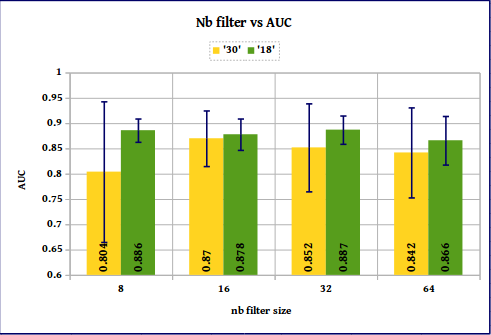
\includegraphics[height=5cm,width=0.5\textwidth]{images/densenet/nb_filter_vs_auc_growthrate_compare}
\caption{Nb\_filter (different growth rates)}
\label{fig:nb_filter_vs_auc_growthrate_compare}
\end{figure}

\subsubsection{Conclusion}
figure \ref{fig:nb_filter_vs_auc} shows that the nb\_filter 16 works better than others and also happen to have the Maximum AUC recorded and lowest standard deviation as well. 
Next it is also curious to know if there is any effect of the growth rate change on the nb filter size. It seems for thinner networks (lower growth rates) it matters lesser than the thicker networks. 
Since for 18 growth rate the mean AUC for all the values of nb\_filter are very close. But there is lot of difference for growth rate 30 for different rates.
However both the networks were found to work pretty good with nb\_filter value of 16. This could have been further evaluated with more growth rates, but for this work we are settling with 16 as our best nb\_filter value.

\subsection{Dropout analysis}
Densenet dropout: 10 evaluations each \\
Mean AUC is best for dropout 0.4\\
Max AUC is highest for dropout 0.5\\
Now it is no surprise that with 0, 0.1 and 0.7 dropouts the results are not the best, because its either too less or too much. But it is bit surprising to have 0.3 and 0.5 performing low. It is out of trend. 

\begin{figure}[ht]
\centering
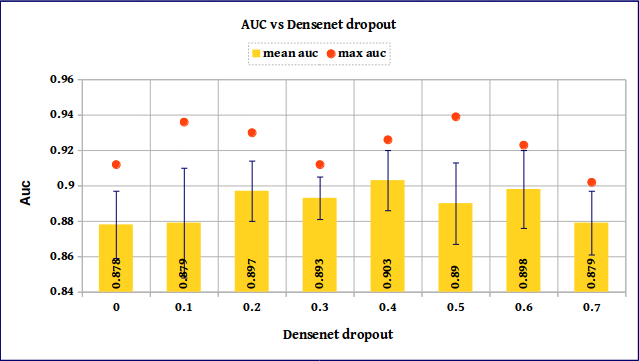
\includegraphics[height=5cm,width=0.5\textwidth]{images/densenet/auc_vs_densenet_dropout}
\caption{Densenet dropout analysis}
\label{fig:auc_vs_densenet_dropout}
\end{figure}
Choosing 0.4 as the dropout rate value for future evaluations.

\subsection{Bottleneck and Compression(also called reduction) analysis}

\begin{figure}[ht]
\centering
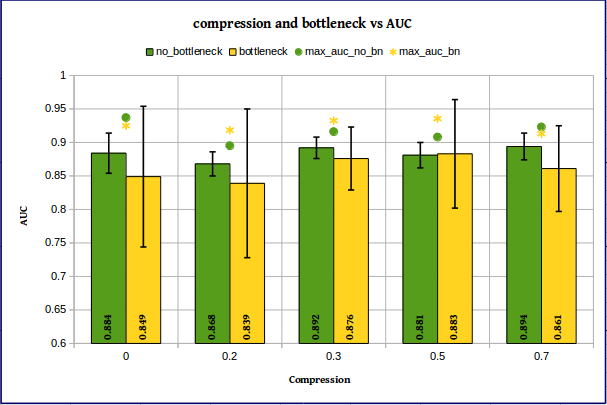
\includegraphics[height=5cm,width=0.6\textwidth]{images/densenet/compression_and_bottleneck_vs_auc}
\caption{Evaluation of compression and bottleneck and mean AUC(across 10 trials). The max AUC obtained by one of the trial is also displayed separately for experiment with bottleneck and without bottleneck.}
\label{fig:compression_and_bottleneck_vs_auc}
\end{figure}

\begin{figure}[ht]
\centering
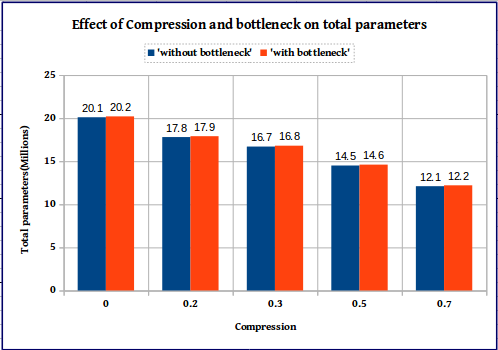
\includegraphics[height=5cm,width=0.5\textwidth]{images/densenet/compression_and_bn_vs_parameters}
\caption{The total parameters are varying with reduction. It also gets affected by use of bottleneck or not, how ever that is very minimal.}
\label{fig:compression_and_bn_vs_parameters}
\end{figure}

\subsubsection{Conclusion}
The use of compression really makes the model much more compact without losing the effectiveness. Without compression the parameter size is 20.1 Millions, after using compression of 0.7 the mean AUC is still as good but 
the size has become 12.1 millions\\
Use of bottleneck does in-fact increase the parameters by little more than 0.1 million, but it does not improve the results at all. So this is a strange behavior.\\ 
Bottleneck also has much higher standard deviation.\\ 
Theoretically it is suppose to help making the model more compact. But over all effects on our data is observed to be adverse.VERY STRANGE!\\
But note: the max auc values still belong to the bottleneck layers 3 out of 5 times. Other two times also its close to highest. That's interesting. 

\subsection{Siamese hyper-parameters analysis}

\begin{wrapfigure}{r}{5cm}
\label{siamese_densenet_structure_wraped}
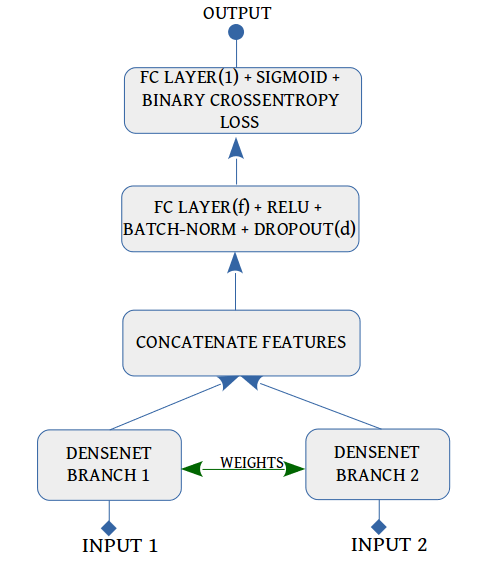
\includegraphics[width=5cm]{images/densenet/siamese_densenet_structure}
\caption{Siamese Densenet Structure}
\end{wrapfigure} 
The concatenated feature maps from the two branches are connected to the fully connected layer before feeding it to the decisive fully-connected layer with 1 output and sigmoid activation.  
%What is the role of this network? todoExplain We ended up here after trial and testing, if this layer is removed then the performance gets very very bad. On the other hand it is interesting to see the effect
%of adding another block of \textbf{FC-RELU-BN} and see the effect. 
\par
The most interesting hyper-parameters associated to the Siamese side, are the fully-connected(FC) layer filter size (f) and the dropout ratio (d) shown in the figure. Everything else is pretty standard.
The fully-connected layers are initialized with “He normal” initialization as they works great with RELU (TODO: add source).
\flushbottom
\newpage
\subsubsection{Fully-connected dropouts analysis}

\begin{figure}[ht]
\centering
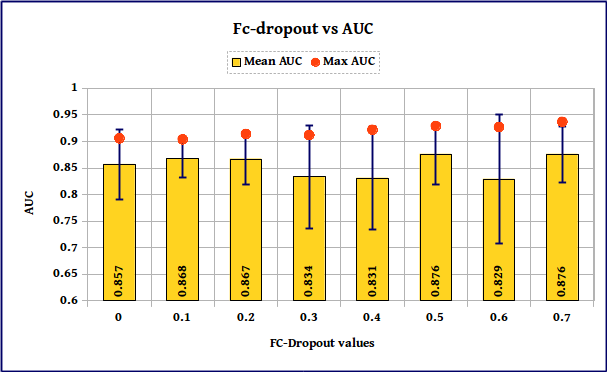
\includegraphics[height=5cm,width=0.5\textwidth]{images/densenet/fc_dropout}
\caption{Optimal dropout (d) for FC layer analysis}
\label{fig:fc_dropout}
\end{figure}

\textbf{Conclusion} 
\begin{itemize}
 \item From figure \ref{fig:fc_dropout} dropouts analysis it seems that the dropout 0.5 has the highest mean AUC along with 0.7. 
 \item The values for 0.3,0.4 is lower than expected and 0.7 is much higher, may be should look for higher dropout values for the analysis.
 %\item TODO: Because of the high std values perhaps an analysis of the 5-number summary can be done here.
\end{itemize}


\subsubsection{Fully-connected network filter size analysis}

\begin{figure}[ht]
\centering
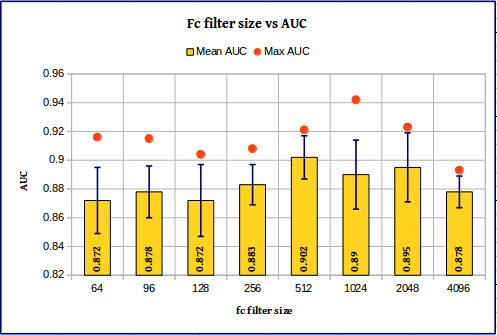
\includegraphics[height=5cm,width=0.5\textwidth]{images/densenet/fc_filter_size}
\caption{optimal FC filter size (f) analysis}
\label{fig:fc_filter_size}
\end{figure}

\textbf{Conclusion} 
\begin{itemize}
 \item The f=512 works the best in terms of the mean AUC (from the graph above). Though the max AUC obtained by the f=1024 and f=2048 is also scoring very good
 \item however on this value of f the number of total parameters for the whole network depends as the whole feature map of each Densenet branch are flattened using “flatten” then concatenated.
 Hence multiplied by 2 (since 2 branches). This concatenated feature map is then multiplied by the f when they gets connected.
  \begin{itemize}
    \item One Densenet branch feature map (size=n) 
    \item Concatenated both branches (size=2n) 
    \item Concatenated features gets connected to fc network with filter size f (2n*f computations, output size = f)
  \end{itemize} 
 \item In other words the smallest f size which gives good performance, is better since it keeps the computations smaller. So f=512 is chosen.
\end{itemize}

\flushbottom
\newpage

\subsection{Batch size analysis}
If the batch size is too low then it takes more time and after a certain size it does not train well too.\\
If the batch size is very big then it may train faster but they generalize lesser as they tend to converge to sharp minimizers of the training function.
TODO add source (https://arxiv.org/abs/1609.04836) 
\begin{figure}[ht]
\centering
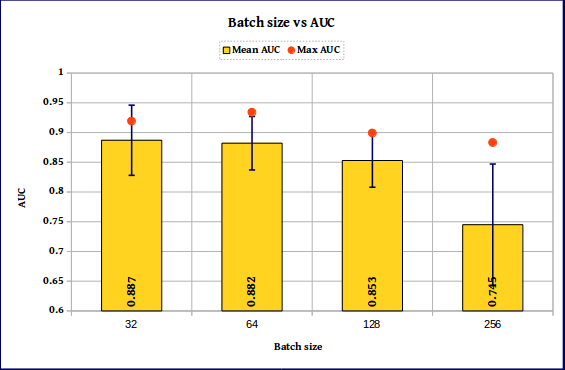
\includegraphics[height=5cm,width=0.5\textwidth]{images/densenet/batch_size}
\caption{Batch size analysis}
\label{fig:batch_size}
\end{figure}

\subsubsection{Conclusion}
From the figure \ref{fig:batch_size} it is evident that the larger the batch size gets the generalization on the test data gets worse. Batch size 32 or 64 looks very close so may be both can be top picks.
The max AUC score for batch size 64 is much higher than others so it is slight favorite though. 


\subsection{Learning rate and optimizer analysis}
\begin{figure}[htp]
\centering
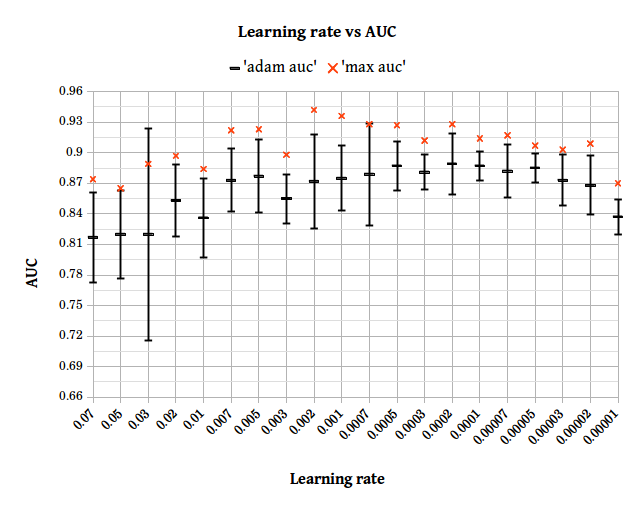
\includegraphics[width=.4\textwidth]{images/densenet/adam_lr}\quad
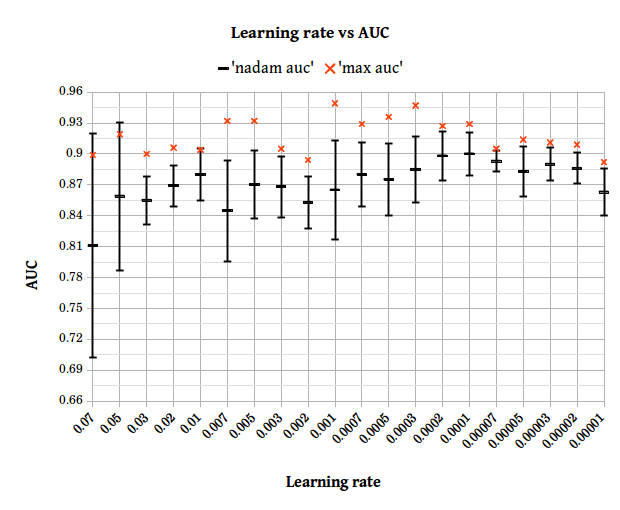
\includegraphics[width=.4\textwidth]{images/densenet/nadam_lr}

\medskip
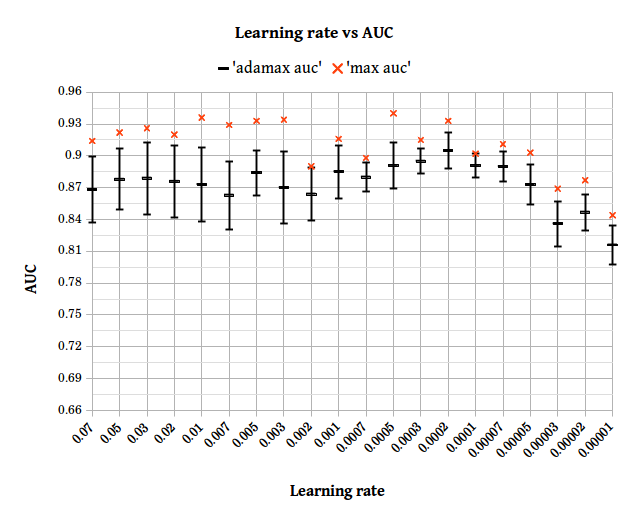
\includegraphics[width=.4\textwidth]{images/densenet/adamax_lr}\quad
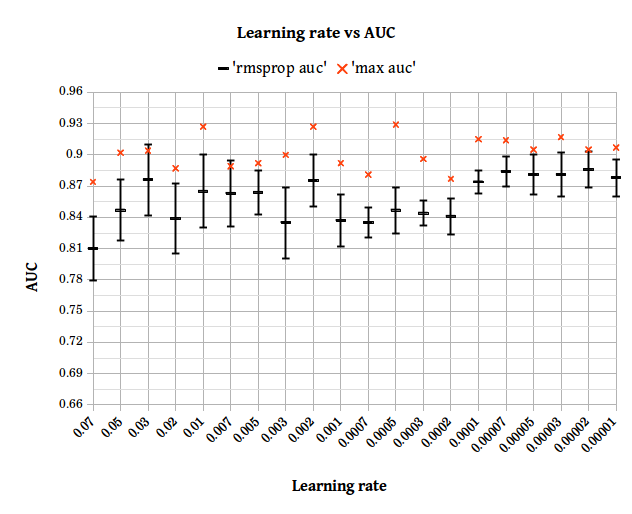
\includegraphics[width=.4\textwidth]{images/densenet/rmsprop_lr}

\medskip
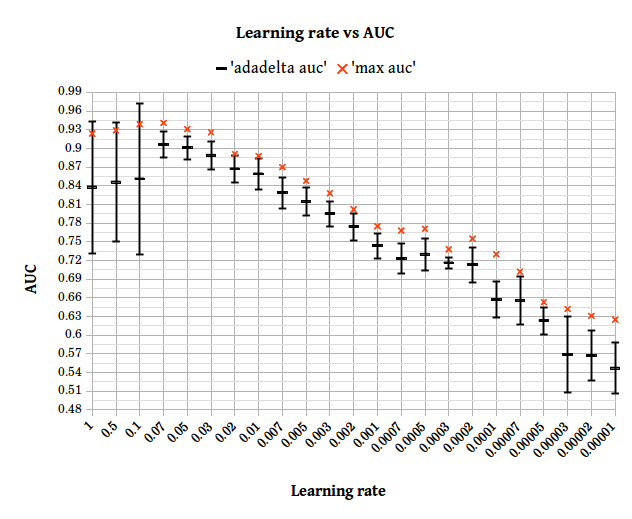
\includegraphics[width=.4\textwidth]{images/densenet/adadelta_lr}

\caption{In order, (a)Adam, (b)Nadam, (c)Adamax, (d)RMSprop, (e)Adadelta learning rate analysis}
\label{pics:lr_optimizers}
\end{figure}

\begin{figure}[htp]
\centering
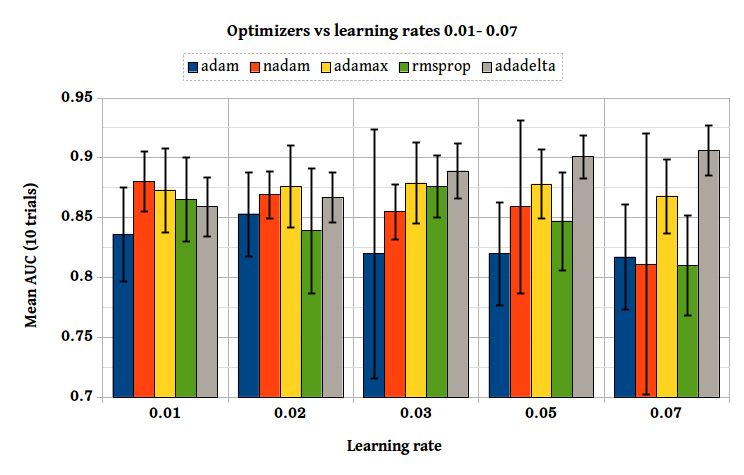
\includegraphics[width=.4\textwidth]{images/densenet/first_compare_lr_opt}\quad
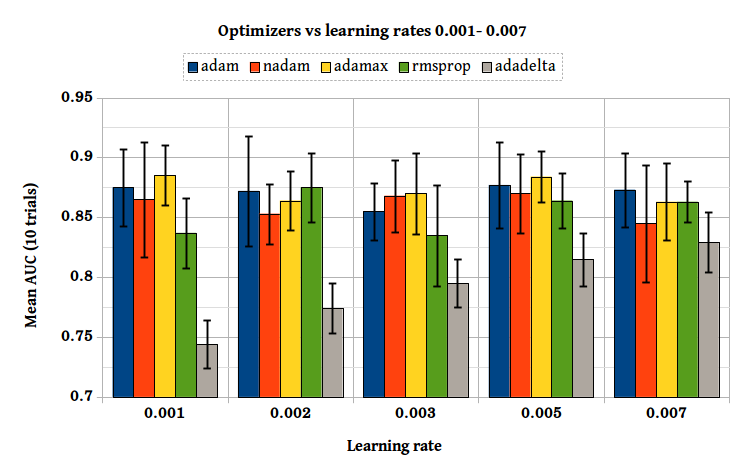
\includegraphics[width=.4\textwidth]{images/densenet/second_compare_lr_opt}

\medskip
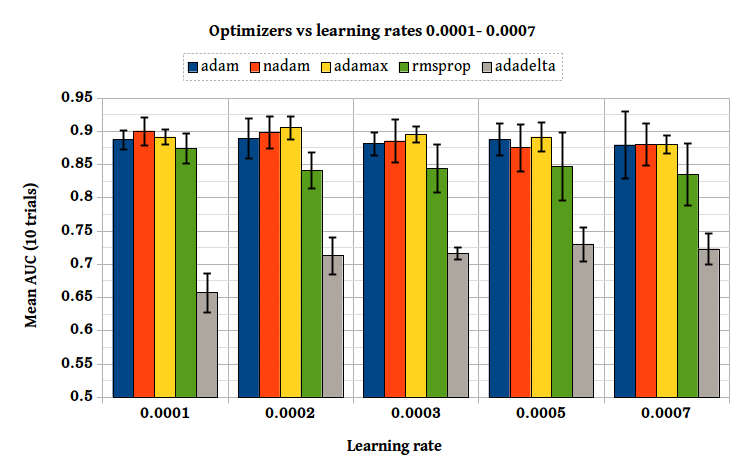
\includegraphics[width=.4\textwidth]{images/densenet/third_compare_lr_opt}\quad
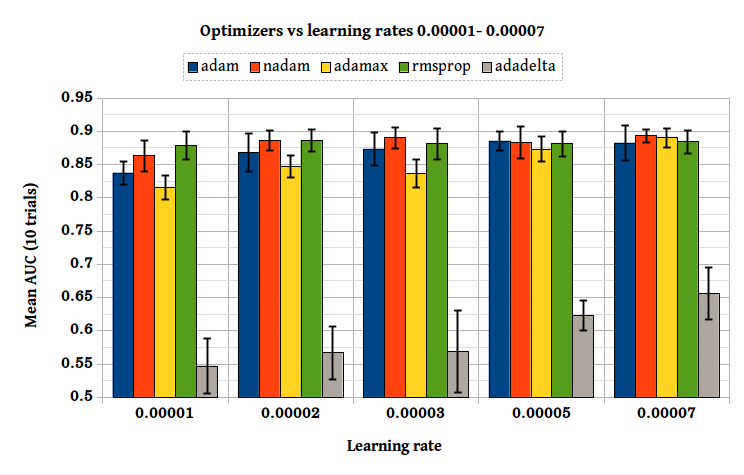
\includegraphics[width=.4\textwidth]{images/densenet/fourth_compare_lr_opt}

\caption{comparison of different optimizers across different learning rates}
\label{pics:lr_optimizers_compare}
\end{figure}
Optimal learning rate selection is very important for effective learning. However, optimal learning rate varies optimizer to optimizer, hence learning rate and optimizer a very fine grained search is performed here
The search space looks as below:
\begin{itemize}
 \item Learning rate:
  \begin{itemize}
    \item 0.01, 0.02, 0.03, 0.05, 0.07
    \item 0.001, 0.002, 0.003, 0.005, 0.007
    \item 0.0001, 0.0002, 0.0003, 0.0005, 0.0007
    \item 0.00001, 0.00002, 0.00003, 0.00005, 0.00007
  \end{itemize}
 \item Optimizers:
 \begin{itemize}
    \item Adam
    \item Nadam
    \item Adamax
    \item RMSprop
    \item Adadelta
 \end{itemize}
\end{itemize}
TODO: Justify choice of the particular optimizers



\subsubsection{Conclusion} 
\begin{itemize}
    \item 10 trials for each test condition
    \item Overall adadelta (lr 0.07) has the highest mean AUC 0.906
    \item highest mean AUC for RMSprop(lr 0.00002) is 0.886
    \item highest mean AUC for Adamax(lr 0.0002) is 0.905
    \item highest mean AUC for Nadam(lr 0.0001) is 0.9
    \item highest mean AUC for Adam(lr 0.0002) is 0.889
    \item So the most effective learning rate varies optimizer to optimizers
    \item For Adamax,Adam,Nadam, lr 0.0002 works very good, for RMSprop lr 2E-5 works better and for Adadelta as the lr drops the performance also drops significantly.
    \item For Adadelta the boundary value for the evaluation is the highest so further analysis needs to be done for higher learning rates like 0.1, 0.5, 1.0. The default learning rate for Adadelta in Keras is 1.0 so it
    is not really surprising.
    \item From figure \ref{fig:adadelta_highlr_analysis} it is observed that each of the trials with learning rate 0.1, 0.5 and 1.0 somehow had 2 AUCs out of 10, which are far lower than others. Which are displayed in 
    the boxplot as the outliers. Without the outliers the average mean of the trials would drastically improve and look as follows. Though we are chosing the 0.07 as the best lr for Adadelta as it is found to be more 
    dependable and high scoring too.
\end{itemize}

\begin{center}
 \begin{tabular}{||c c c c c||} 
 \hline\hline
 Learning rate & 0.07 & 0.1 & 0.5 & 1.0 \\ [0.5ex] 
 \hline
 Mean AUC & 0.906 & 0.906 & 0.891 & 0.887 \\ 
 \hline
\end{tabular}
\end{center}

\begin{figure}[htp]
\centering
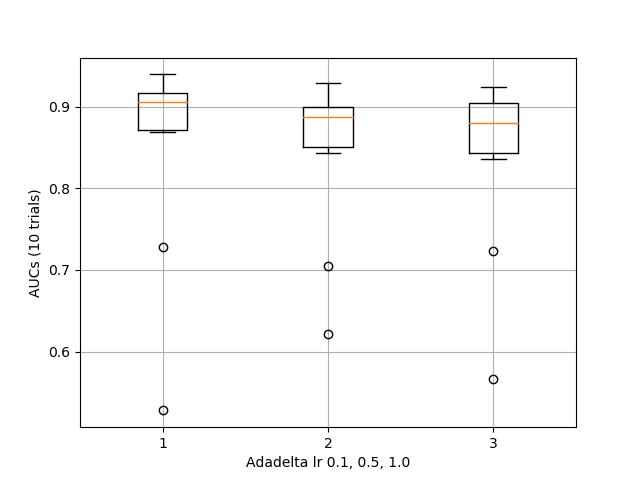
\includegraphics[height=3.5cm]{images/densenet/adadelta_highlr_analysis}
\caption{Adadelta advance learning rate analysis}
\label{fig:adadelta_highlr_analysis}
\end{figure}

\subsection{Hyper-parameters for final grid search}
\begin{itemize}
 \item Layers per block 2-2, 3-4
 \item nb\_dense\_block 2
 \item Growth rate 12, 18, 30
 \item Nb\_filter 16
 \item Densenet dropout 0.2, 0.4
 \item Bottleneck False
 \item Compression 0.3, 0.7
 \item FC filter size 512
 \item FC dropout 0.5, 0.7
 \item Learning rate 0.0002 and optimizer Adamax, Learning rate 0.07 optimizer Adadelta, Learning rate 0001 optimizer Nadam
 \item Batch size: 64
\end{itemize}

\subsection{Best results in final grid search(as of now)}
\textbf{Top config 1 Adadelta}\\
Epochs  14  batch\_size:  64  lr:  0.07  optimizer: adadelta \\
es\_patience:  4  lr\_patience:  3\\
batch\_size:  64  fc\_dropout:  0.7  fc\_filter:  512  fc\_layers:  1 \\
Layers:  [2, 2]  Growth\_rate:  30  \\
nb\_filter:  16  dropout:  0.4 dense\_block  2  \\
reduction\_:  0.3  bottleneck:  False \\

\textbf{Top config 2 Adadelta}\\
Epochs  13  batch\_size:  64  lr:  0.07  optimizer:  adadelta \\
es\_patience:  4  lr\_patience:  3\\
batch\_size:  64  fc\_dropout:  0.7  fc\_filter:  512 fc\_layers:  1\\
Layers:  [2, 2]  Growth\_rate:  12 nb\_filter:  16  dropout:  0.2 
dense\_block  2 reduction\_:  0.7  bottleneck:  False

\textbf{Top config 3 Adamax}\\
Epochs  14  batch\_size:  64  lr:  0.0002  optimizer:  adamax \\
 es\_patience:  4  lr\_patience:  3\\
 batch\_size:  64  fc\_dropout:  0.7  fc\_filter:  512  fc\_layers:  1 \\
Layers:  [3, 4]  Growth\_rate:  12  nb\_filter:  16  dropout:  0.4 \\
dense\_block  2  reduction\_:  0.7  bottleneck:  False \\

\textbf{Top config 4 Adamax}\\
Epochs  15  batch\_size:  64  lr:  0.0002  optimizer:  adamax\\
 es\_patience:  4  lr\_patience:  3 \\
 batch\_size:  64  fc\_dropout:  0.7  fc\_filter:  512  fc\_layers:  1 \\
Layers:  [2, 2]  Growth\_rate:  18  nb\_filter:  16  dropout:  0.4 \\
dense\_block  2  reduction\_:  0.7  bottleneck:  False\\

\textbf{Top config 5 Nadam}\\
Epochs  13  batch\_size:  64  lr:  0.0001  optimizer:  nadam\\
 es\_patience:  4  lr\_patience:  3 \\
 batch\_size:  64  fc\_dropout:  0.7  fc\_filter:  512  fc\_layers:  1\\
Layers:  [3, 4]  Growth\_rate:  30  nb\_filter:  16  dropout:  0.4\\
dense\_block  2  reduction\_:  0.3  bottleneck:  False

%Divide this into three tables as well for densenet for fc + normal
%\begin{center}
% \begin{tabular}{||c c c c c c c c c c c c c c c c c||} 
% \hline\hline
% Layers & Growth\_rate & dense\_block & nb\_filter & dropout & reduction\_ & bottleneck & fc\_dropout & fc\_filter & Epochs & batch\_size & lr & optimizer & es\_patience & lr\_patience & batch\_size \\ [0.5ex] 
% \hline
% 0.608 & 0.854 & 0.881 & 0.902 & 0.934 & 3 & 0.608 & 0.854 & 0.881 & 0.902 & 0.934 & 3 & 0.608 & 0.854 & 0.881 & 0.902 & 0.934 \\ 
% \hline
% 0.608 & 0.854 & 0.881 & 0.902 & 0.934 & 3 & 0.608 & 0.854 & 0.881 & 0.902 & 0.934 & 3 & 0.608 & 0.854 & 0.881 & 0.902 & 0.934 \\
% \hline
%\end{tabular}
%\end{center}

\begin{figure}[ht]
\centering
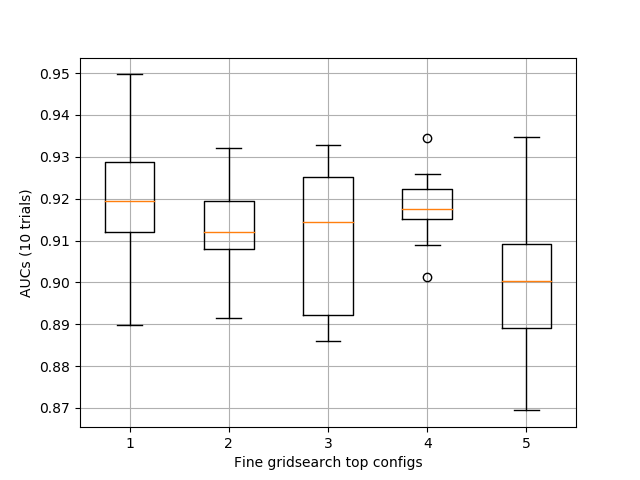
\includegraphics[height= 5cm]{images/densenet/fine_grid_search_top_configs}
\caption{Fine grid search top results}
\label{fig:fine_grid_search_top_configs}
\end{figure}

\begin{figure}[ht]
\centering
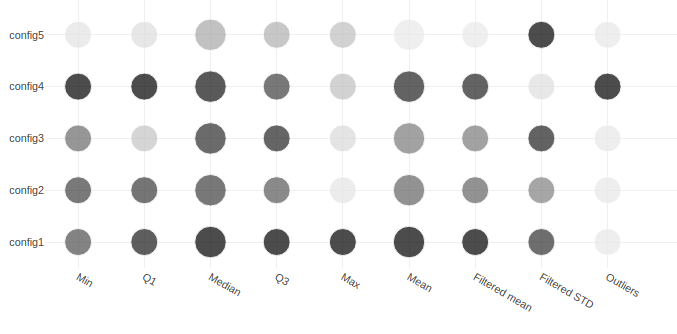
\includegraphics[height= 4cm]{images/densenet/top5_analysis_bubble}
\caption{Fine grid search top results statistical analysis}
\label{fig:top5_analysis_bubble}
\end{figure}

%\flushbottom
%\newpage

\subsubsection{Conclusion}
\begin{itemize}
 \item State of the art highest AUC \textbf{0.91}
 \item Densenet Siamese: Highest mean AUC across 10 trials were for Adadelta with learning rate 0.07. \textbf{Mean AUC: 0.921 STD: 0.016 Max AUC: 0.950}
 \item The mean result for the top configs are very close and it is hard to declare a runaway winner as the highest network has mean AUC of .921 and std of 0.016, second best has mean AUC of 0.918 with std 0.005. 
 \item Top Config 4 interestingly has outliers, both high and low. 
 \item It is interesting to note that the dropout values which are giving the best results are high 0.7 for the Siamese side and 0.4 for the densenet side. 
 \item High dropout and Batch normalization is enabling the network to be good in generalization. The training/validation accuracy is could reach 99\% still the test AUC score is high enough.
 %\item Is it fair to calculate outliers in auc analysis?
 \item The statistical comparison of the top 5 performing runs are displayed below in figure \ref{fig:fine_grid_search_top_configs}
 \item In figure \ref{fig:top5_analysis_bubble} multiple statistical data is displayed in bubbles whose color indicates the scale of the value. Lower values indicated by lighter shade of grey. The highest value is shown 
 in black. The scale of the shades are normalized between highest and lowest values for each column. But the white was not visible so for each cases the minimum was lowered little bit so the lowest value is very light grey 
 not white. TODO this needs further finnese. %TODO find better colormap
 %\item Is it fair to calculate mean AUC after excluding the outliers? Not it is unfair
\end{itemize}




